\documentclass[
    table,
    12pt,
    oneside,
    a4paper,
    italian
]{book}

\PassOptionsToPackage{dvipsnames}{xcolor} % colori PDF/A

\usepackage{colorprofiles}
% PDF/A
% validate in https://www.pdf-online.com/osa/validate.aspx
\usepackage[a-1a,mathxmp]{pdfx}[2018/12/22]
\usepackage[T1]{fontenc}
\usepackage[utf8]{inputenc}
\usepackage[italian]{babel}
\usepackage{bookmark}
\usepackage{caption}
\usepackage{comment}
\usepackage{chngpage, calc} % centra il frontespizio
\usepackage{emptypage} % pagine vuote senza testatina e piede di pagina
\usepackage{epigraph} % per epigrafi
\usepackage{indentfirst} % rientra il primo paragrafo di ogni sezione
\usepackage{graphicx} % immagini
\usepackage[pdfa]{hyperref} % collegamenti ipertestuali
\usepackage{mparhack,relsize}  % finezze tipografiche
\usepackage{nameref} % visualizza nome dei riferimenti
\usepackage[font=small]{quoting} % citazioni
\usepackage{subfig} % sottofigure, sottotabelle
\usepackage[italian]{varioref} % riferimenti completi della pagina
\usepackage{longtable} % tabelle su più pagine
\usepackage[toc, acronym, automake]{glossaries}
\usepackage[backend=biber, style=verbose-ibid, hyperref, backref]{biblatex}
\usepackage{lmodern}
\usepackage[top=2.75cm, bottom=2.75cm, right=3cm, left=3.75cm]{geometry} % 1in+17pt+0.6cm
\usepackage{fancyhdr}
\usepackage{lipsum}
\usepackage{setspace}
\usepackage{titlesec}
\usepackage[cachedir=minted-caches]{minted} % https://it.overleaf.com/learn/latex/Code_Highlighting_with_minted
\usepackage{xcolor}
\usepackage{csquotes} % gestisce automaticamente i caratteri (")
\usepackage{etoolbox}
\usepackage[bottom]{footmisc}
\usepackage{zref-totpages}
% Load variables
\newcommand{\myUni}{Università degli Studi di Padova}
\newcommand{\myDepartment}{Dipartimento di Matematica ``Tullio Levi-Civita''}
\newcommand{\myFaculty}{Corso di Laurea in Informatica}
\newcommand{\myTitle}{MoviORDER, modulo agenti per gestione clienti}
\newcommand{\myDegree}{Tesi di Laurea Triennale}
\newcommand{\profTitle}{Prof.}
\newcommand{\myProf}{Vardanega Tullio}
\newcommand{\graduateTitle}{Laureando}
\newcommand{\myName}{Oseliero Antonio}
\newcommand{\myStudentID}{1226325}
\newcommand{\myAA}{2023-2024}
\newcommand{\myLocation}{Padova}
\newcommand{\myTime}{Settembre 2024}
% Acronyms
%\newacronym{api}{API}{Application Program Interface}
%\newacronym{sdk}{SDK}{Software Development Kit}

% Glossary
\newglossaryentry{api}{
    name={API},
    text={API},
    sort=api,
    description={ \textit{Application Programming Interface} (interfaccia di programmazione delle applicazioni) sono un insieme di definizioni 
    e protocolli con i quali vengono realizzati e integrati \textit{software applicativi}. Le API stabiliscono il contenuto e la forma dei dati 
    necessari per la chiamata e quelli restituiti in risposta.\\
    {[\textit{fonte riportata in sitografia}]}}
}

\newglossaryentry{csr}{
    name={CSR},
    text={CSR},
    sort=csr,
    description={   
                    Per Responsabilità Sociale delle Imprese (e delle organizzazioni) o secondo l'acronimo inglese CSR, 
                    \textit{Corporate Social Responsibility}, si intende l'integrazione su base volontaria, da parte delle imprese, 
                    delle preoccupazioni sociali e ambientali nelle loro operazioni interessate.\\
                    {[\textit{fonte riportata in sitografia}]}}
}

\newglossaryentry{erp}{
    name={ERP},
    text={ERP},
    sort=erp,
    description={
                    \textit{Enterprise Resource Planning}, è un tipo di sistema \textit{software} che aiuta le organizzazioni ad automatizzare e 
                    gestire i processi aziendali principali per ottenere le prestazioni ottimali. Il \textit{software} ERP coordina il flusso di dati 
                    tra i processi di un'azienda, fornendo un'unica fonte di informazioni e semplificando le operazioni nell'azienda. È in grado di 
                    collegare le attività finanziarie, della catena di approvvigionamento, delle operazioni, del commercio, dei \textit{report}, della 
                    produzione e delle risorse umane di un'azienda in una sola piattaforma.\\
                    {[\textit{fonte della definizione inglese riportata in sitografia}]}}
}

\newglossaryentry{ide}{
    name={IDE},
    text={IDE},
    sort=ide,
    description={
                    \textit{Integrated Development Environment} o ambiente di sviluppo integrato, è un \textit{software} progettato per la 
                    realizzazione di applicazioni che aggrega strumenti di sviluppo comuni in un'unica interfaccia utente grafica. In genere è costituito da: 
                    \textit{editor} del codice sorgente, strumenti che consentono di automatizzare la \textit{build} locale, un \textit{debugger} e 
                    strumenti per l'esecuzione di test automatici.\\
                    {[\textit{fonte riportata in sitografia}]}}
}

\newglossaryentry{webapp}{
    name={Web App},
    text={web app},
    sort=webapp,
    description={
                    L'applicazione \textit{web}, o abbreviato \textit{web app}, nell'ambito dell'informatica e della programmazione, 
                    si riferisce alle applicazioni accessibili e fruibili attraverso il \textit{web}, quindi accessibili dall'utente 
                    tramite un \textit{browser web} con una connessione attiva
                }
}



% Define custom colors
\definecolor{hyperColor}{HTML}{0B3EE3}
\definecolor{tableGray}{HTML}{F5F5F7}
\definecolor{veryPeri}{HTML}{6667ab}

% Set line height
\linespread{1.5}

% Custom hyphenation rules
\hyphenation {
    data-base
    al-go-rithms
    soft-ware
}

% Images path
\graphicspath{{img/}}

% Force page color, as some editors set a grayish color as default
\pagecolor{white}

% Better spacing for footnotes
\setlength{\skip\footins}{5mm}
\setlength{\footnotesep}{5mm}

\setlength{\headheight}{14.5pt}
\addtolength{\topmargin}{-2.45pt}

% Add a subscript G to a glossary entry
\newcommand{\glox}{\textsubscript{\textbf{\textit{G}}}}

% Improvements the paragraph command
\titleformat{\paragraph}
{\normalfont\normalsize\bfseries}{\theparagraph}{1em}{}
\titlespacing*{\paragraph}
{0pt}{3.25ex plus 1ex minus .2ex}{1.5ex plus .2ex}

% Define use case environment
\newcounter{usecasecounter} % define a counter
\setcounter{usecasecounter}{0} % set the counter to some initial value
% Parameters
% #1: ID
% #2: Nome
\newenvironment{usecase}[2]{
    \renewcommand{\theusecasecounter}{\usecasename #1}  % this is where the display of the counter is overwritten/modified
    \refstepcounter{usecasecounter} % increment counter
    \vspace{2em}
    \par \noindent % start new paragraph
    {\normalsize \textbf{\usecasename #1: #2}} % display the title before the content of the environment is displayed
    \vspace{.5em}
}{
    \medskip
}
\newcommand{\usecasename}{UC}
\newcommand{\usecaseactors}[1]{\textbf{\\Attori Principali:} #1}
\newcommand{\usecasepre}[1]{\textbf{\\Precondizioni:} #1}
\newcommand{\usecasedesc}[1]{\textbf{\\Descrizione:} #1}
\newcommand{\usecasepost}[1]{\textbf{\\Postcondizioni:} #1}
\newcommand{\usecasealt}[1]{\textbf{\\Scenario Alternativo:} #1}

% Define risks environment
\newcounter{riskcounter} % define a counter
\setcounter{riskcounter}{0} % set the counter to some initial value
% Parameters
% #1: Title
\newenvironment{risk}[1]{
    \refstepcounter{riskcounter} % increment counter
    \par \noindent % start new paragraph
    \textbf{\arabic{riskcounter}. #1} % display the title before the content of the environment is displayed
}{
    \par\medskip
}
\newcommand{\riskname}{Rischio}
\newcommand{\riskdescription}[1]{\textbf{\\Descrizione:} #1.}
\newcommand{\risksolution}[1]{\textbf{\\Soluzione:} #1.}

% Apply fancy styling to pages
\pagestyle{fancy}
\fancyhf{}
\fancyhead[L]{\leftmark} % Places Chapter N. Chatper title on the top left
\fancyfoot[C]{\thepage} % Page number in the center of the footer

% Adds a blank page while increasing the page number
\newcommand\blankpage{ 
\clearpage
    \begingroup
    \null
    \thispagestyle{empty}
    \hypersetup{pageanchor=false}
    \clearpage
\endgroup
}

% Adds a blank page while increasing the page number
\newcommand\blankpagewithnumber{ 
  \clearpage
  \thispagestyle{plain} % Use plain page style to keep the page number
  \null
  \clearpage
}

% Increase page numbering
\newcommand\increasepagenumbering{
    \addtocounter{page}{+1}
}

% Make glossaries and bibliography
\makeglossaries
% Redefine the format for the glossary entries to be italic
\renewcommand*{\glstextformat}[1]{\textit{#1}\glox}
%\glsaddall

\bibliography{references/bibliography}
\defbibheading{bibliography} {
    \cleardoublepage
    \phantomsection
    \addcontentsline{toc}{chapter}{\bibname}
    \chapter*{\bibname\markboth{\bibname}{\bibname}}
}

% Code blocks handling w/ table of codes
\makeatletter
\ifdefined\NR@chapter
  \expandafter\@firstoftwo
\else
  \expandafter\@secondoftwo
\fi{\patchcmd\NR@chapter}{\patchcmd\@chapter}
  {\addtocontents{lot}{\protect\addvspace{10\p@}}}
  {\addtocontents{lot}{\protect\addvspace{10\p@}}%
   \addtocontents{lol}{\protect\addvspace{10\p@}}}
  {}{}
\makeatother

\renewcommand\listingscaption{Codice}
\renewcommand\listoflistingscaption{Elenco dei codici sorgenti}
\counterwithin*{listing}{chapter}
\renewcommand\thelisting{\thechapter.\arabic{listing}}

% Set up hyperlinks
\hypersetup{
    colorlinks=true,
    linktocpage=true,
    pdfstartpage=1,
    pdfstartview=,
    breaklinks=true,
    pdfpagemode=UseNone,
    pageanchor=true,
    pdfpagemode=UseOutlines,
    plainpages=false,
    bookmarksnumbered,
    bookmarksopen=true,
    bookmarksopenlevel=1,
    hypertexnames=true,
    pdfhighlight=/O,
    allcolors = hyperColor
}

% Set up captions
\captionsetup{
    tableposition=top,
    figureposition=bottom,
    font=small,
    format=hang,
    labelfont=bf
}

% When draft mode is on, the hyperlinks are removed. Useful when printing the document. To enable/disable, uncomment/comment the command
% \hypersetup{draft}

% prevents cleaning up the cache at the end of the run (needed to keep the unused caches, generated by other editions)
\makeatletter
\renewcommand*{\minted@cleancache}{}
\makeatother

% Break lines in code blocks whe using inputminted
\setminted{breaklines}

\date{}

\usepackage{indentfirst}
\setlength{\parindent}{0pt}

\hypersetup{pdfstartview=}
\begin{document}
    \frontmatter
    \begin{titlepage}
    \begin{center}
        \begin{Large}
            \textbf{\myUni}\\
        \end{Large}

        \vspace{5pt}

        \begin{large}
            \textsc{\myDepartment}\\
        \end{large}

        \vspace{5pt}

        \begin{large}
            \textsc{\myFaculty}\\
        \end{large}

        \vspace{25pt}
        
        \begin{figure}[htbp]
            \centering
            
\includegraphics[alt={Emblema dell'Università degli Studi di Padova}, height=6cm]{img/logo_unipd.jpeg}
        \end{figure}

        
        \begin{Large}
            \textbf{\myTitle}\\
        \end{Large}

        \vspace{5pt}

        \begin{large}
            \textit{\myDegree}\\
        \end{large}

        \vspace{50pt}
        
        \begin{normalsize}
            \begin{flushleft}
                \textit{Relatore}\\
                \profTitle\ \myProf
            \end{flushleft}

            \vspace{-48pt}
            
            \begin{flushright}
                \textit{\graduateTitle}\\
                \myName\\
                Matricola \myStudentID
            \end{flushright}
        \end{normalsize}

        \vspace*{\fill}
        
        \line(1, 0){338} \\
        \begin{normalsize}
            \textsc{Anno Accademico \myAA}
        \end{normalsize}
    \end{center}
\end{titlepage}

    \increasepagenumbering % increase the page numbrering by 1, in order to cout the frontispiece
    \clearpage
\phantomsection
\thispagestyle{empty}
\hfill
\vfill

{\small\noindent\textcopyright\ \myName, \myTime. Tutti i diritti riservati. \myDegree: ``\textit{\myTitle}'', \myUni, \myDepartment.}
    %\chapter*{Ringraziamenti}

Desidero esprimere la mia più profonda gratitudine al professor {\myProf}, per la sua supervisione attenta e la sua
guida esperta, che hanno contribuito ad elevare la qualità di questa tesi.\\
Ringrazio sinceramente il mio tutor aziendale, {\myTutor}, amministratore di {\company}, per il suo inestimabile 
supporto durante lo \textit{stage} e per l'opportunità concessami di lavorare in azienda. Estendo i miei 
ringraziamenti all'intero \textit{team} di {\company} per la calorosa accoglienza e l'assistenza costante 
durante la mia esperienza di tirocinio.\\
Un sentito ringraziamento va ai miei compagni di corso, con cui ho condiviso questo percorso 
universitario.\\
Esprimo la mia gratitudine alla mia famiglia per il loro sostegno durante tutto il mio percorso 
di studi, e ai miei amici per il loro costante incoraggiamento.

\vspace{0.75cm}

\noindent{\myLocation, \myTime}
\hfill \textit{\myName}



    \cleardoublepage
\phantomsection
\pdfbookmark{Compendio}{Compendio}
\begingroup
\let\clearpage\relax
\let\cleardoublepage\relax
\chapter*{Sommario}

Il presente documento descrive il lavoro svolto dallo studente {\myName} durante il suo stage presso l’azienda {\companyLong}.\\
Lo scopo del tirocinio è stato studiare il codice dell’applicazione mobile {\movi} e sviluppare un modulo di autenticazione di agenti aziendali 
in un'applicazione pensata per clienti terzi. Più precisamente era richiesto che, dopo l’autenticazione, l’agente possa scegliere un cliente da una 
lista e operare all’interno dell’applicazione come il cliente selezionato senza la necessità di autenticarsi come tale.\\
Raggiungere questo obiettivo ha richiesto lo studio del codice e dell’architettura dell’applicazione: \textbf{\textit{front-end, back-end} e base dati 
sottostante}, e un certo insieme di tecnologie e strumenti tra i quali \textbf{React Native e ASP.NET Core, Visual Studio, e Server Management Studio}. 
Il progetto ha incluso la realizzazione delle API e l’interfaccia grafica del modulo richiesto, insieme a una batteria di test automatici per la 
\textit{Business Logic} di alcune di tali API.\\\\

All'interno del documento tutte le parole inglesi verranno segnalate in \textit{corsivo}.\\
Per i termini che fanno riferimento a tabelle e colonne del database, classi, funzioni, component, view o altre parti del 
codice verrà utilizzato il carattere \texttt{monospaziato}.\\
Le parole facenti parte del glossario saranno evidenziate tramite una G a pedice, il corsivo e la parola sarà di colore blu (esempio \gls{csr}).\\
Nel documento verrà utilizzato il \textbf{grassetto} per enfatizzare la parola chiave di un punto di un elenco puntato o il singolo elemento di un elenco. 
Questo per migliorare la leggibilità del documento e rendere subito identificabili i concetti chiave di una lista.\\
Ad esempio una lista sarà cosi visualizzata:\\
"i numeri primi sono \textbf{1,2,3,7}...", \\
mentre un elenco puntato apparirà nel seguente modo:\\
"elenco numeri primi:
\begin{itemize}
    \item \textbf{1};\item \textbf{2};\item \textbf{3};
\end{itemize}
..."\\\\


Il documento è diviso in 4 macro sezioni:\\
\textbf{Capitolo 1 - VisioneImpresa}: descrizione dell'azienda in cui ho svolto il tirocinio riportando brevemente clienti, prodotti, organizzazione aziendali, strumenti e 
tecnologie utilizzate, propensione dell'azienda all'innovazione;\\
\textbf{Capitolo 2 - Descrizione e pianificazione stage}: qui si riporta il progetto assegnatomi dall'azienda riportando obiettivi, vincoli tecnologici e temporali, viene 
inoltre approfondito il rapporto dell'azienda con gli stage in generale e la motivazione dietro la scelta di questo specifico progetto;\\
\textbf{Capitolo 3 - Stage}: descrizione della mia esperienza di stage;\\
\textbf{Capitolo 4 - Retrospettiva}: giudizio obiettivo in merito il soddisfacimento degli obiettivi di stage, personali e aziendali, oltre 
ad un resoconto delle conoscenze acquisite con questa esperienza e una personale valutazione del percorso di studi universitario.


\endgroup
\vfill

    \cleardoublepage
\pdfbookmark{\contentsname}{tableofcontents}
\setcounter{secnumdepth}{5}
\setcounter{tocdepth}{5}     

\tableofcontents
\clearpage

\begingroup
    \let\clearpage\relax
    \let\cleardoublepage\relax
    \let\cleardoublepage\relax

    % Figures list
    \phantomsection
    \pdfbookmark{\listfigurename}{lof}
    \listoffigures
    \vspace*{8ex}

    % Tables list
    \phantomsection
    \pdfbookmark{\listtablename}{lot}
    \listoftables
\endgroup

\begingroup
    % Code list
    \phantomsection
    \pdfbookmark{\listoflistingscaption}{lol}
    \listoflistings
\endgroup

\cleardoublepage
    
    \blankpage % example of a blank page that also increases the page couter by 1

    \mainmatter
    \chapter{VisioneImpresa}\label{chap:VisioneImpresa}

\section{L'azienda}
{\company} è un'azienda con quarant'anni di esperienza nell'offrire a piccole e medie imprese soluzioni informatiche per la 
gestione e l'automazione dei processi aziendali. I suoi prodotti di punta sono infatti sistemi \gls{erp} (\textit{Enterprise 
Resource Planning}) ovvero sistemi che permettono di coordinare il flusso di dati tra i processi di un'azienda, fornendo un'unica fonte di 
informazioni e semplificandone le operazioni.\\
{\company} è situata a Pernumia (Padova) e opera in prevalenza nel Nord Est, dal 2016 è entrata a far parte del gruppo Officegroup, azienda 
che riunisce diverse \textit{software house} specializzate nella progettazione e sviluppo di sistemi gestionali evoluti. 
Dal 2023 inoltre è diventata una società \textit{benefit}, ovvero è un azienda che opera con l'obiettivo di generare un impatto positivo 
sulla società e sull'ambiente, oltre al profitto finanziario.

\begin{figure}[H]
    \centering
    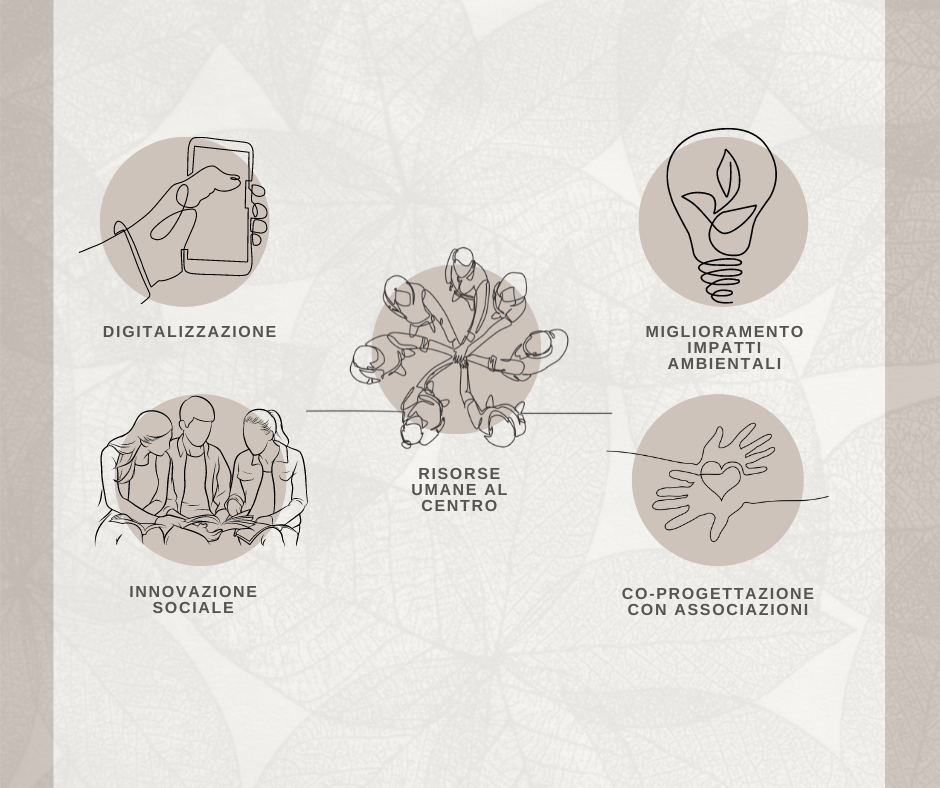
\includegraphics[alt={Obiettivi delle società benefit}, width=0.5\textwidth]{img/soc-benefit.png}
    \caption[Obiettivi delle società benefit.]{Obiettivi delle società benefit. \\ \textit{fonte: https://www.vsh.it/azienda/societa-benefit/}}
    \label{fig:società benefit}
\end{figure}

Come mostrato in Figura \ref{fig:società benefit} questo tipo di società attuano iniziative in diversi ambiti, dalla dematerializzazione 
e digitalizzazione alla promozione di politiche a sostegno della conciliazione vita-lavoro.\\
Altri obiettivi delle società \textit{benefit} possono essere: investire nelle \textbf{energie rinnovabili e la sostenibilità}, l'investimento in \textbf{tecnologie 
ad alta efficienza energetica}, rispetto della \textbf{parità di genere}, \textbf{formazione professionale} del lavoratore, \textbf{progetti con scuole ed 
università, co-progettazione con associazioni e istituzioni del territorio} con il duplice obiettivo di stimolare la partecipazione dei dipendenti 
a “buone cause” della comunità e \textbf{valorizzare il lavoro di associazioni no-profit} del territorio, generando così valore sociale.


\section{Clienti e servizi}
{\company} ha come clienti piccole e medie imprese situate in prevalenza in Veneto e in generale nel Nord Italia, possiamo trovare però 
anche clienti dal Centro Italia e dalla Sardegna. \\
Il gestionale che propone può adattarsi a qualsiasi tipo di azienda indipendentemente dal settore in cui 
operi (anche se come vedremo vengono venduti dei gestionali ad hoc per i settori: petrolifero, ittico, assistenza post-vendita, ortofrutticolo, antincendi 
e antinfortunistica, trasporti).\\ Una volta implementato il gestionale all'interno dell'azienda del cliente viene offerta una formazione all'utilizzo del 
\textit{software} per i dipendenti, che parteciperanno a delle riunioni tenute da un consulente tecnico che ne illustrerà le funzionalità e insegnerà come sfruttarle 
al meglio.\\
{\company} propone due linee di prodotti principali: Vision e MoviDAT.
La prima, Vision, è la linea di gestionali dell'azienda, con VisionENTERPRISE, che è il loro \gls{erp} di punta, 
e poi una serie di soluzioni verticali per venire incontro alle specifiche esigenze delle varie aziende con cui {\company} opera.
Ognuna delle soluzioni verticali offerte dall'azienda è una variazione di VisionENTERPRISE, che viene arricchita con 
funzionalità specifiche per adattarsi a specifici settori. In particolare quindi nella linea Vision abbiamo:
\begin{itemize}
      \item \textbf{VisionENTERPRISE}, \gls{erp} di punta dell'azienda e dedicato ad imprese che non hanno necessità di funzionalità 
      specifiche.
      \item \textbf{VisionENERGY}, gestionale con specifiche funzionalità pensate per le aziende che lavorano nel settore petrolifero, 
      come la possibilità di gestire la vendita di carburante, manutenzione valvole, ecc.;
      \item \textbf{VisionBLUE}, gestionale con specifiche funzionalità pensate per le aziende che lavorano nel settore ittico, 
      come la possibilità di gestire lotti, prodotti e imballaggi;
      \item \textbf{VisionASSISTANCE}, gestionale con specifiche funzionalità pensate per le aziende specializzate nell'assistenza post-vendita, 
      come la possibilità di gestire richieste di assistenza, contratti e assegnare gli ordini di intervento ai 
      singoli tecnici;
      \item \textbf{VisionFRESH}, gestionale con specifiche funzionalità pensate per le aziende che lavorano nel settore ortofrutticolo, 
      come la possibilità di gestire movimentazione merce, inserimento pesate, interfacciamento con bilance elettroniche, ecc.;
      \item \textbf{VisionANTINCENDI}, gestionale con specifiche funzionalità pensate per le aziende che lavorano nel settore antincendi e antinfortunistica, 
      come la possibilità di gestire chiamate ed interventi straordinari, buoni di manutenzione e geolocalizzare gli interventi;
      \item \textbf{VisionTRASPORTI}, gestionale con specifiche funzionalità pensate per le aziende che lavorano nel settore trasporti, 
      come la possibilità di gestire listini, anagrafiche, dotazioni, manutenzione, pianificazione viaggi, ecc.
\end{itemize}
Nella linea di prodotti MoviDAT invece troviamo una gamma di applicazioni sviluppate per i principali sistemi operativi per dispositivi 
\textit{mobile}: Android e iOS. Queste applicazioni sono state sviluppate per integrarsi direttamente con i gestionali 
della linea Vision e permettono di semplificare il lavoro di dipendenti che operano in mobilità e non hanno a disposizione un 
\textit{computer} con cui lavorare durante le trasferte (ed anche se ce lo avessero il suo utilizzo risulterebbe scomodo).\\
In questa linea dunque troviamo:
\begin{itemize}
    \item \textbf{MoviDOC} è un \gls{webapp} (ovvero un \textit{app} a cui è possibile accedere direttamente da \textit{browser} senza 
          necessità di installarla sul dispositivo) che consente la gestione e condivisone dei documenti;
    \item \textbf{Handy} è un \textit{app} per palmare che integrata a VisionENTERPRISE supporta la movimentazione della merce del magazzino o del punto vendita;
    \item \textbf{MoviSELL} è un \textit{app} sviluppata per \textit{tablet} iOS dedicata agli agenti aziendali, permette di: visualizzare i 
          clienti su una mappa, avere visibilità dello stato contabile e inserire ordini clienti direttamente nel 
          ciclo attivo dell'azienda.
    \item \textbf{MoviREP} è un \textit{app} sviluppata per \textit{tablet} iOS per la gestione digitalizzata dei rapportini da parte di operatori addetti alla manutenzione o 
          all'assistenza post vendita. 
    \item \textbf{MoviALERT} è una \gls{webapp} che permette di inviare \textit{mail} di notifica automatiche all'avvenire di 
          specifici eventi nel gestionale;
    \item \textbf{MoviCHECK} è un \gls{webapp}, scaricabile anche su dispositivi Android e iOS per 
          consultare i dati di business in mobilità;
    \item \textbf{MoviEXPENSE} è un \textit{app} per Android e iOS, per la registrazione automatica delle note 
          spese;
    \item \textbf{MoviCHECKIN} è una \gls{webapp} per la registrazione dei visitatori in azienda;
    \item \textbf{MoviORDER} applicazione per \textit{smartphone e tablet} iOS e Android che l’azienda può fornire ai propri clienti per l’invio di ordini e 
          richieste di approvvigionamento.
\end{itemize}

Nel caso in cui un'azienda richieda funzionalità specifiche per uno dei \textit{software} sopra elencati, {\company} offre la possibilità di creare una versione 
modificata dei propri prodotti. Per evitare di avere troppe variazioni della stesso prodotto il codice delle personalizzazioni (così vengono chiamate le funzioni in 
più richieste dal cliente) vengono inserite direttamente nel codice del \textit{software} principale, e "attivate" da specifici parametri controllati all'avvio del 
sistema. Nel caso di MoviORDER, che ho avuto la possibilità di esaminare per questo progetto, a seconda del valore del campo \textit{Company} ottenuto a seguito dell'
autenticazione del cliente venivano apportate alcune variazioni grafiche (loghi, tema). Questo si può ottenere grazie ad un'attenta progettazione e appropriate scelte 
architetturali.

 
\section{Organizzazione aziendale}
\subsection{Aree di competenza}
{\company} è strutturata in tre aree di competenza, ognuna con ruoli e responsabilità specifiche.\\
\textbf{Reparto Assistenza}: qui operano i consulenti tecnici gestionali, il cui compito è assistere l'azienda nell'implementazione dei nuovi gestionali 
e nella gestione del cambiamento assicurandosi che il personale aziendale sia formato sull'uso delle nuove tecnologie. Ogni consulente è responsabile di uno 
o più \textit{software} di cui hanno un ampia conoscenza operativa. Inoltre, forniscono assistenza ai clienti, aiutandoli 
nella risoluzione dei problemi e, se necessario, segnalando le problematiche al reparto sviluppo che aprirà quindi un 
\textit{ticket} all'interno della piattaforma Jira (vedi capitolo \ref{chap:Tecnologie}).\\
\textbf{Area Amministrazione Commerciale e \textit{Marketing}}: In quest'area si trovano diverse competenze, tra cui:
\begin{itemize}
    \item \textbf{Responsabile \textit{marketing}}: ha il compito di realizzare strategie per promuovere l'azienda 
          e i suoi prodotti ai potenziali clienti;
    \item \textbf{Risorse umane}: ha il compito di amministrare stipendi, pensioni e \textit{benefit}, nonché di assicurarsi il rispetto da parte 
          dell'azienda delle normative sul lavoro;
    \item \textbf{Contabilità}: ha il compito di gestire e registrare le transazioni finanziarie, garantendo che tutte le attività economiche 
          siano documentate in modo accurato e trasparente;
    \item \textbf{Segreteria generale}: ha il compito di gestire e indirizzare le chiamate in entrata, gestire la posta elettronica e la 
          corrispondenza, pianificare eventi aziendali;
    \item \textbf{Segreteria commerciale}: ha il compito di mantenere le comunicazioni con i clienti fornendo informazioni su prodotti e 
          servizi e preparando offerte commerciali, contratti di vendita e documenti correlati;
    \item \textbf{Amministrazione ciclo attivo}: ha il compito di garantire una gestione efficiente delle vendite e della riscossione dei pagamenti;
    \item \textbf{Commerciale rete diretta}: ha il compito di occuparsi della vendita dei prodotti direttamente ai clienti finali;
    \item \textbf{commerciale rete indiretta}: ha il compito di gestire le vendite attraverso intermediari come distributori, rivenditori, agenti o partner commerciali;
    \item \textbf{Responsabile d'impatto}: si occupa della valutazione, pianificazione e promozione delle misure di responsabilità sociale d'impresa 
          (\gls{csr}), ovvero di tutte le iniziative attuate dall'azienda in ambito sociale e di transizione ecologica.
    \item \textbf{Amministratore} è responsabile di dirigere e gestire l'azienda nel suo complesso, assicurando che tutti i dipartimenti e le attività 
          lavorino insieme per raggiungere gli obiettivi strategici e operativi.
    \item \textbf{\textit{Product manager}} ha il compito di assicurare che i prodotti siano sviluppati in linea con le esigenze del mercato, lanciati con
          successo e gestiti efficacemente durante il loro ciclo di vita.
\end{itemize}
\textbf{Reparto Sviluppo \textit{Software}}: In quest'area troviamo:
\begin{itemize}
    \item \textbf{Sviluppatori}: possono essere \textbf{\textit{frontend}}, specializzati nello sviluppo di interfacce e della gestione dell'
          interazione uomo-macchina, \textbf{\textit{backend}} specializzati nello sviluppo della logica del \textit{software} e nella manipolazione dei 
          dati, o \textbf{\textit{fullstack}}, in grado di operare sia come sviluppatore \textit{frontend} che \textit{backend}.
    \item \textbf{\textit{Project manager}}: ha il compito di assicurarsi che vengano rispettati obiettivi, tempi, costi e vengano soddisfatti
          i parametri di qualità;
    \item \textbf{Direttore dello sviluppo}: ha il compito di prendere le decisioni implementative e scegliere l'architettura del \textit{software}, si 
          occupa inoltre di dirigere il team e di pianificare e assegnare i lavori da svolgere;
    \item \textbf{Analista}: si occupa di interagire con i clienti per delineare i requisiti del progetto \textit{software} e documentarli in un documento 
          di analisi.
\end{itemize}

\subsection{Metodologie di sviluppo \textit{software}}
Ho potuto notare, durante la mia esperienza di tirocinio, che gli sviluppatori utilizzano metodologie Agile per la gestione dei loro progetti.\\
Le metodologie Agile sono un'approccio alla gestione dei progetti che prevede la suddivisione del progetto 
in fasi e del lavoro in cicli brevi, al termine dei quali verranno introdotti cambiamenti che avvicinano il 
progetto sempre di più al soddisfacimento di tutti i requisiti. Questo approccio è particolarmente adattabile agli imprevisti, permettendo di reagire velocemente 
e riducendo al minimo i danni, come lo slittamento della data di completamento e conseguentemente l'aumento di denaro da destinare al progetto. 
Il manifesto Agile riporta i punti principali punti di questa filosofia:
\begin{itemize}
      \item Gli \textbf{individui e le interazioni} più che i processi e gli strumenti;
      \item Il \textbf{software funzionante} più che la documentazione esaustiva;
      \item La \textbf{collaborazione col cliente} più che la negoziazione del contratto;
      \item \textbf{Rispondere al cambiamento} più che seguire un piano.
\end{itemize}
In particolare, {\company} adotta il \textit{framework} Agile Scrum, che definisce una 
serie di principi, pratiche e cerimonie per riuscire ad assimilare nel proprio metodo di lavoro la metodologia Agile. 
Scrum richiede di suddividere il lavoro in \textit{sprint} dalla durata variabile di una fino a quattro settimane. {\company} pianifica
sprint di una settima in modo da rispondere tempestivamente a gli imprevisti ed effettuare una pianificazione più efficace.

\begin{figure}[H]
      \centering
      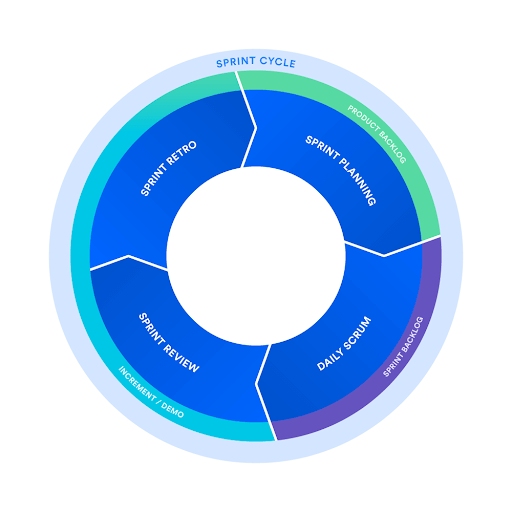
\includegraphics[alt={Organizzazione di uno sprint con il \textit{framework} Scrum}, width=0.5\textwidth]{img/scrum.png}
      \caption[Organizzazione di uno sprint con il \textit{framework} Scrum]
              {Organizzazione di uno sprint con il \textit{framework} Scrum. \\ \textit{fonte: https://www.atlassian.com/it/agile/scrum}}
      \label{fig:scrum}
  \end{figure}

Come mostrato in Figura \ref{fig:scrum} ogni sprint è strutturato in una serie di incontri che avvengono solitamente in video chiamata usando 
3CX (vedi capitolo \ref{chap:Tecnologie}).\\ 
Si comincia il lunedì, all'inizio dello \textit{sprint}, quando programmatori, direttore dello sviluppo e \textit{project manager} partecipano 
ad un \textit{meeting} chiamato \textit{sprint planning} dove si pianifica il lavoro da svolgere per lo sprint in corso.
Quindi ogni giorno si tiene un breve \textit{meeting} prima della pausa pranzo chiamato \textit{daily scrum} dove si discute dello stato dei lavori ed 
eventuali problemi emersi.
Il venerdì si tiene l'ultimo \textit{meeting} dello \textit{sprint} chiamato \textit{sprint review} dove si discute 
dello stato dei lavori rispetto alle aspettative e discutendo dei problemi emersi durante lo \textit{sprint} si cercano modi per migliorare.\\
{\company} organizza inoltre un ulteriore \textit{meeting} a cadenza mensile dove non solo le persone interessate al progetto, ma tutti i dipendenti dell'azienda 
si riuniscono per discutere dello stato dei lavori di ogni settore: \textbf{evoluzione dei prodotti, vendite, feedback dei clienti, aggiornare il reparto \textit{marketing}
 e commerciale sulle nuove funzionalità dei software ecc.}. Questo incontro ha 
lo scopo di dare a tutti i dipendenti dell'azienda una visione d'insieme evitando il cosiddetto "effetto sottomarino", ovvero quando una persona o un gruppo si focalizzano 
soltanto in uno specifico ambito, favorendo l'isolamento rispetto al resto dell'azienda, che ha invece bisogno di lavorare coordinando i vari settori.
\section{Tecnologie}\label{chap:Tecnologie}
\subsection{Elenco delle tecnologie utilizzate}
L'azienda utilizza diversi strumenti sia per lo sviluppo, che per lo svolgimento dei normali processi aziendali.
\begin{itemize}
    \item \textbf{Portatili}: ad ogni impiegato viene messo a disposizione un portatile con Windows 10 o 11, il sistema 
          operativo di Microsoft o all'occorrenza un Mac con macOS, il portatile sviluppato da Apple con il suo sistema operativo proprietario;
    \item \textbf{Dispositivi \textit{mobile}}: all'interno dell'azienda troviamo molti dispositivi \textit{mobile} con diversi sistemi operativi e dimensioni 
          dello schermo, usati per il \textit{testing} delle applicazioni Android e iOS;
    \item \textbf{Microsoft Office 365}: servizio in abbonamento di Microsoft che include diversi software come Word e PowerPoint;
    \item \textbf{Zimbra}: sistema di posta elettronica utilizzato dall'azienda, durante il mio stage è stato cambiato in favore di un'integrazione di Zimbra 
          con Outlook;
    \item \textbf{Bitbucket}: strumento per la gestione della versione Git basato sul \textit{web}, che consente di creare 
          \textit{repository} pubbliche o private per caricare il proprio codice e gestirlo in modo collaborativo con il proprio 
          \textit{team};
    \item \textbf{Jira}: \textit{suite} di \textit{software} proprietari per il tracciamento delle segnalazioni sviluppato
           da Atlassian, che consente il \textit{bug tracking} e la gestione dei progetti;
    \item \textbf{Confluence}: strumento che permette ai \textit{team} di condividere e organizzare documenti e contenuti 
          in un ambiente centralizzato e strutturato;
    \item \textbf{3CX}: centralino telefonico PBX (\textit{Private Branch Exchange}), ovvero una rete telefonica privata utilizzata all'interno di un'azienda 
          o organizzazione. Gli utenti del sistema telefonico PBX possono comunicare internamente ed esternamente, tramite il classico telefono fisso o 
          chat da \textit{smartphone}. Questo sistema permette anche di effettuare video chiamate e di scambiarsi messaggi all'interno di \textit{chat};
    \item \textbf{Visual Studio}: Si tratta di un ambiente di sviluppo integrato completo (\gls{ide}) che è possibile usare per scrivere, modificare, 
          eseguire il \textit{debug} e compilare codice. Visual Studio include \textbf{compilatori, strumenti di completamento del codice, 
          controllo del codice sorgente, estensioni} e molte altre funzionalità per migliorare ogni fase del processo di sviluppo \textit{software};
    \item \textbf{Visual Studio Code}: \textit{editor} di codice sorgente particolarmente leggero ed estensibile grazie ad una gamma di estensioni 
          che è possibile integrargli. È inoltre \textit{open source} e compatibile con una vasta gamma di sistemi operativi;
    \item \textbf{SQL Server Management Studio (SSMS)}: è un ambiente integrato per la configurazione, la gestione e l'amministrazione di tutti i componenti, 
          le istanze e i database all'interno di Microsoft SQL Server. SSMS include sia \textit{editor} di \textit{script} che strumenti grafici che lavorano con 
          oggetti e funzionalità del \textit{server}.
    \item \textbf{Swagger}: un insieme di strumenti e tecnologie per la progettazione, la costruzione e la documentazione delle \gls{api} RESTful, ovvero delle interfacce 
          che permettono a i vari \textit{software} di comunicare tra loro.
\end{itemize}
L'azienda utilizza una vasta gamma di linguaggi di programmazione, \textit{framework} e librerie per diversi motivi. Alcuni di questi includono l'acquisizione 
e l'adattamento di codice sorgente da altre aziende, il fatto che il codice sia stato scritto molti anni fa con tecnologie ormai obsolete, e la necessità di utilizzare 
linguaggi specifici per soddisfare esigenze particolari. Tuttavia, l'azienda si impegna a uniformare quanto più possibile i linguaggi e a ridurre il numero di tecnologie in 
uso, al fine di semplificare e rendere più efficiente la gestione delle risorse tecnologiche. Oltre a quelle che ho usato per il mio progetto (che verranno discusse 
più approfonditamente nel capitolo TODO 2.4.1) queste sono alcune delle tecnologie che l'azienda usa per lo sviluppo dei suoi prodotti.
\begin{itemize}
    \item \textbf{Angular}: \textit{framework} per lo sviluppo di \gls{webapp} basato su TypeScript, sviluppato e mantenuto da Google;
    \item \textbf{Librerie Dev Express}: Dev Express è un'azienda incentrata sulla creazione di librerie di componenti grafici di cui le più famose sono 
          Blazor e MAUI. Queste librerie sono supportate per lo sviluppo in React, Angular e Vue;
    \item \textbf{FoxPro}: un sistema di gestione di \textit{database} e un linguaggio di programmazione procedurale orientato agli oggetti. Originariamente sviluppato 
          da Fox Software e successivamente acquisito da Microsoft. 
\end{itemize}
\subsection{Integrazione delle tecnologie con i processi aziendali}
\begin{figure}[H]
      \centering
      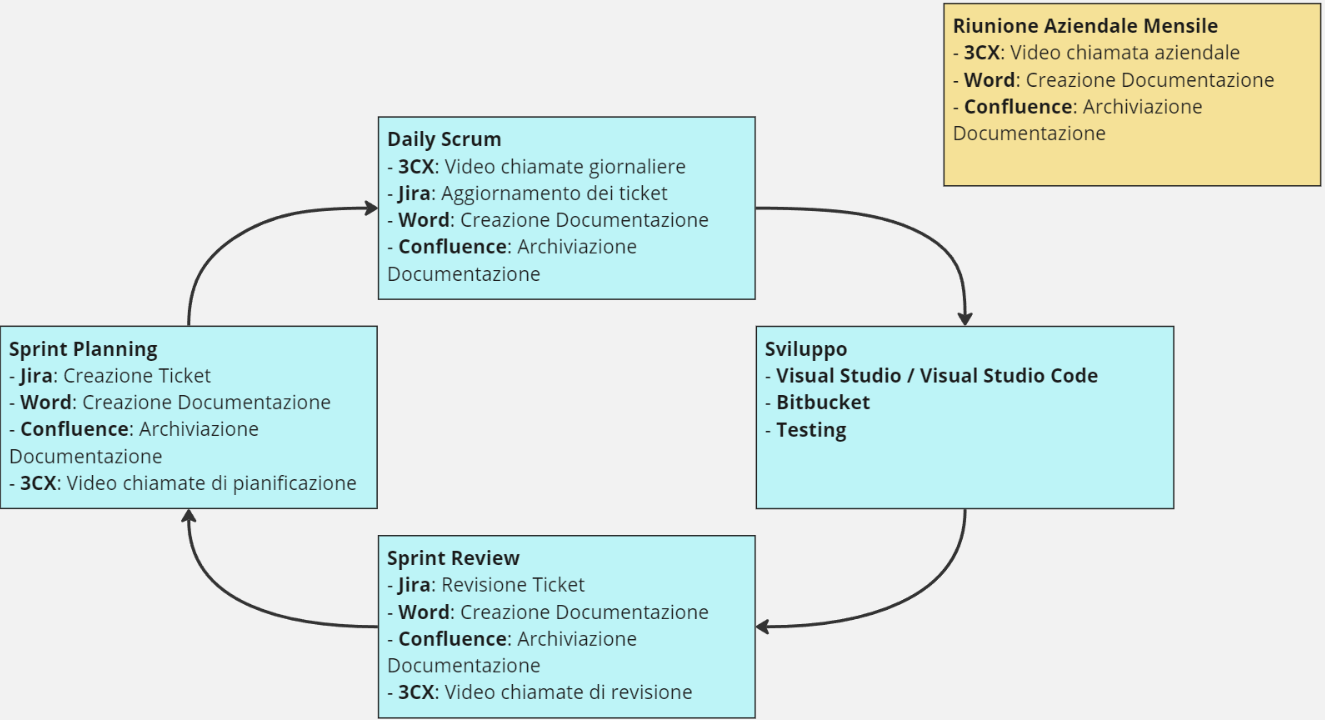
\includegraphics[alt={metodologie e tecnologie}, width=\textwidth]{img/integrazione metodologie strumenti.png}
      \caption[Integrazione metodologie e tecnologie]
              {Integrazione metodologie e tecnologie.}
      \label{fig:integrazione tecnologie e metodologie}
  \end{figure}
Come mostrato in figura \ref{fig:integrazione tecnologie e metodologie} l'applicazione del \textit{framework} Scrum richiede 
l'impiego di diverse tecnologie:
\begin{itemize}
      \item \textbf{Documentazione}: a seguito dei \textit{meeting} aziendali viene prodotto un documento che può 
            avere diverse finalità: trascrivere gli \textbf{argomenti dell'incontro}, le \textbf{difficoltà incontrate e le soluzioni da 
            applicare per correggerle} o \textbf{semplici appunti}. Gli sviluppatori usano quindi Word per redarre la documentazione 
            data la sua estrema semplicità e la velocità con la quale si possono produrre tali documenti;
      \item \textbf{Archiviazione di documenti}: eccezion fatta per gli appunti personali, la documentazione richiede di 
            essere condivisa e organizzata. Nonostante in {\company} esista una serie di cartelle di rete accedibili tramite 
            il \textit{file manager} di Windows, questa soluzione risulta inadeguata allo scopo in quanto povera di funzionalità 
            e personalizzazioni. Confluence permette non solo di organizzare la documentazione in una serie di \textit{directory 
            online} in modo da rendere i documenti sempre consultabili, ma permette anche di definire una serie di privilegi per 
            consentire o meno l'accesso alla documentazione.
      \item \textbf{Comunicazione}: 3CX agisce come canale di comunicazione per la maggior parte delle comunicazioni interne. 
            È il luogo dove si svolgono i \textit{meeting}, fondamentali per mantenere il \textit{team} coordinato, ma permette 
            anche di effettuare chiamate e scrivere in \textit{chat} confinando la maggior parte delle comunicazioni in un unico 
            luogo. Ovviamente anche le \textit{mail} sono un valido strumento di comunicazione, ed infatti viene usato Zimbra 
            per comunicare con persone esterne all'azienda o per alcune mail interne (\textbf{comunicazioni di servizio, 
            \textit{reminder}}, ecc.). Quindi 3CX viene usato maggiormente per i \textit{meeting} o per un tipo di 
            comunicazione veloce ed informale, mentre il servizio di posta elettronica viene usato principalmente 
            per comunicazione con persone esterne all'azienda. Ovviamente i clienti che hanno necessità di assistenza 
            possono chiamare l'assistenza tramite il numero di telefono che viene loro fornito per mettersi in contato con 
            uno dei tecnici del reparto assistenza;
      \item \textbf{Sviluppo}: Per quanto riguarda lo sviluppo gli strumenti utilizzati e le tecnologie impiegate variano 
            a seconda del progetto a cui lo sviluppatore sta lavorando o da preferenze personali (come nel caso del 
            sistema operativo utilizzato nel proprio \textit{computer}). Anche per quanto riguarda l'editor viene lasciata 
            libertà di scelta, personalmente per lo sviluppo di \gls{api} in .NET (le tecnologie che ho impiegato per lo sviluppo del 
            progetto verranno discusse in un capitolo a parte TODO 3.1) ho preferito utilizzare Visual Studio perché offre 
            molti strumenti di supporto e \textit{debug} integrati. Per quanto riguarda lo sviluppo del \textit{front-end} ho 
            preferito utilizzare Visual Studio Code perché più leggero, personalizzabile.
      \item \textbf{Testing}: anche qui gli strumenti utilizzati dipendono dal progetto che si sta sviluppando. Nel mio 
            caso ho utilizzato uno \textit{smartphone e tablet} Android per testare l'applicazione nel suo insieme e la 
            piattaforma Swagger per testare manualmente le \gls{api} (le tecnologie che ho impiegato per lo sviluppo del 
            progetto verranno discusse in un capitolo a parte TODO 3.1, mentre per la descrizione accurata di come ho 
            effettuato il testing del codice consultare il capitolo TODO 3.6). Riporto per completezza che per 
            quanto riguarda il \textit{testing} di applicazioni Android è possibile emulare un dispositivo con gli 
            strumenti offerti dallo strumento di sviluppo Android Studio e installare l'applicazione su questo \textit{device} 
            virtuale. Il problema di questo strumento è che richiede computer con prestazioni molto alte per funzionare 
            in maniera fluida altrimenti rischia di paralizzare l'elaboratore. Non sono sicuro che sia utilizzato dagli 
            sviluppatori di {\company} quindi ho evitato di includerlo nelle tecnologie utilizzate;
      \item \textbf{Collaborazione e gestione del codice}: Bitbucket viene utilizzato come piattaforma per depositare il codice 
            sorgente e gestire lo sviluppo collaborativo. Qui gli sviluppatori caricano il loro 
            codice suddiviso in \textit{repository} per ogni progetto. Ogni \textit{repository} vede diversi 
            \textit{branch} attivi: \textbf{\textit{main}} che contiene l'ultima versione rilasciata al pubblico del software, 
            \textbf{\textit{develop}} ovvero il \textit{branch} di lavoro dove nascono e confluiscono tutti i 
            \textit{feature branch} prima di effettuare il rilascio in \textit{main}, i \textbf{\textit{feature branch}} che 
            viene creato dal programmatore per sviluppare una specifica funzione del programma che sarà, una volta 
            terminata e testata, aggiunta in \textit{develop};
      \item \textbf{Gestione dei progetti}: Jira è una piattaforma particolarmente utile per pianificare i vari 
            compiti da svolgere nello \textit{sprint} e assegnarli ai vari componenti del \textit{team} di sviluppatori. 
            Questi compiti sono chiamati \textit{ticket} e possono essere di diverso tipo: \textbf{\textit{epic}} che rappresentano 
            grosse porzioni di lavoro e sono quindi usate come raccolte di \textit{ticket}, \textbf{\textit{task}} il singolo 
            compito che deve essere completato e \textbf{\textit{bug}} che rappresenta una problematica da risolvere.
            I \textbf{\textit{bug}} possono essere avere diverse origini: gli sviluppatori stessi nel caso in cui si accorgano 
            di un difetto di programmazione o da i clienti che telefonando all'assistenza riportano il problema, 
            quindi il tecnico riporterà la problematica al \textit{project manager} che creerà la \textit{task}. Jira offre inoltre 
            molti altri strumenti per la gestione di metodologie Agile come la possibilità di creare diagrammi di Gantt, che 
            permettono di avere una rappresentazione visiva delle attività programmate nel tempo, aiutando il \textit{team} 
            a comprendere meglio la sequenza delle attività, o la definizione di un \textit{backlog}, ovvero una lista con le task 
            rimaste incompiute durante gli \textit{sprint} precedenti;
\end{itemize}
\section{Propensione all'innovazione}\label{chap:Propensione all'innovazione}
{\company} non dispone di un ufficio specificamente dedicato alla ricerca e sviluppo, ma questo non significa che non 
vengano effettuati aggiornamenti costanti delle tecnologie e degli strumenti utilizzati. Ad esempio, l'azienda ha 
in programma di migrare i propri sistemi \gls{erp}, attualmente scritti in FoxPro (un linguaggio il cui supporto da 
parte di Microsoft è terminato nel 2015), verso tecnologie più moderne. Questo progetto, data la grandezza e 
complessità dei software coinvolti, richiederà anni per essere completato.\\
Inoltre, l'attività di stage rappresenta un'opportunità per l'azienda di innovare. Durante il mio tirocinio, 
ho osservato un apprezzamento particolare per l'indipendenza degli stagisti nel cercare e implementare 
soluzioni o tecnologie originali. Per ulteriori dettagli sul rapporto dell'azienda con gli stage, consultare il 
capitolo TODO 2.1.


%\begin{itemize}
%	\item gli acronimi, le abbreviazioni e i termini ambigui o di uso non comune menzionati vengono definiti nel glossario, situato alla fine del presente documento;
%	\item per la prima occorrenza dei termini riportati nel glossario viene utilizzata la seguente nomenclatura: \gls{apig};
%	\item i termini in lingua straniera o facenti parti del gergo tecnico sono evidenziati con il carattere \textit{corsivo}.
%\end{itemize}

\newpage

    \pagenumbering{roman}
    \backmatter
    %\printglossary[type=\acronymtype, title=Acronimi e abbreviazioni, toctitle=Acronimi e abbreviazioni]
    \printglossary[type=main, title=Glossario, toctitle=Glossario]
    %\chapter{Bibliografia}
\label{cap:bibliography}

\nocite{*}

% Books bibliography
\printbibliography[heading=subbibliography, title={Testi}, type=book]

% Articles bibliography
\printbibliography[heading=subbibliography, title={Articoli}, type=article]

% Websites bibliography
%\printbibliography[heading=subbibliography, title={Siti}, type=online]

    %\chapter{Sitografia}
\label{cap:webliography}
\nocite{*}

% Websites bibliography
\printbibliography[heading=subbibliography, title={\null}, type=online]

\end{document}